\documentclass{standalone}
\usepackage{graphicx}	
\usepackage{amssymb, amsmath}
\usepackage{color}

\usepackage{tikz}
\usetikzlibrary{intersections, backgrounds, patterns, patterns.meta}
\usepackage{pgfmath}

\definecolor{light}{RGB}{220, 188, 188}
\definecolor{mid}{RGB}{185, 124, 124}
\definecolor{dark}{RGB}{143, 39, 39}
\definecolor{highlight}{RGB}{180, 31, 180}
\definecolor{gray10}{gray}{0.1}
\definecolor{gray20}{gray}{0.2}
\definecolor{gray30}{gray}{0.3}
\definecolor{gray40}{gray}{0.4}
\definecolor{gray60}{gray}{0.6}
\definecolor{gray70}{gray}{0.7}
\definecolor{gray80}{gray}{0.8}
\definecolor{gray90}{gray}{0.9}
\definecolor{gray95}{gray}{0.95}

\begin{document}

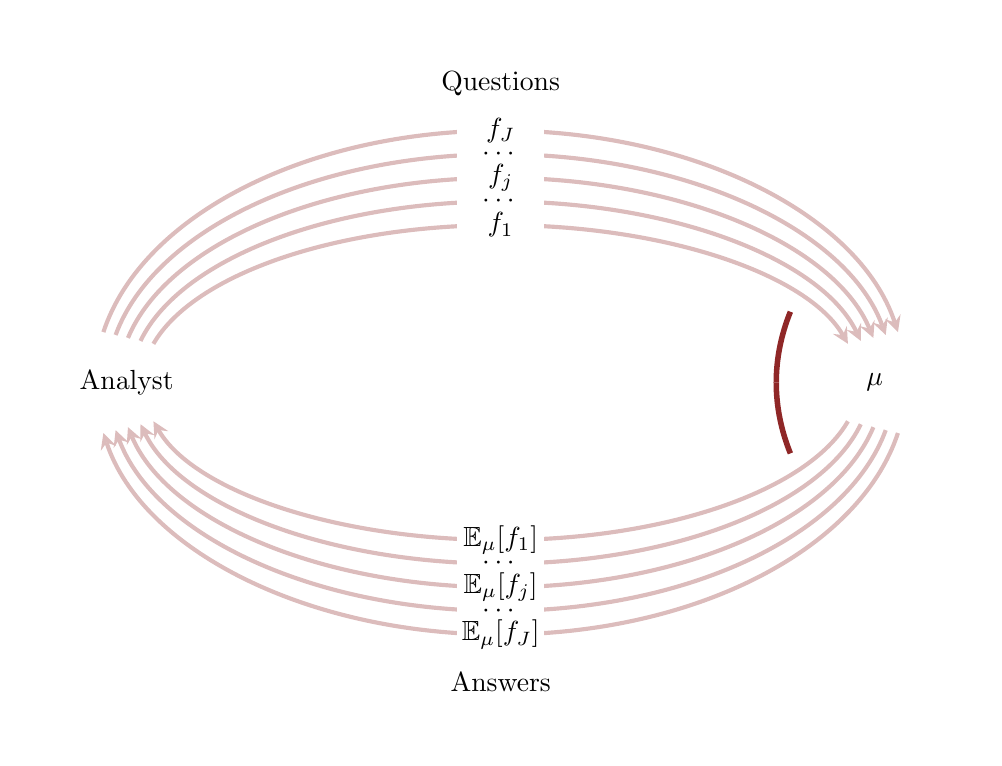
\begin{tikzpicture}[scale=1]

\begin{scope}[shift={(0, 0)}]
  \draw[white] (-6, -4.5) rectangle (6, 4.5);
  
  %\draw[dark] (16, 0) circle (10 and 12);
  \draw[dark, line width=2] (3.5, 0) arc[start angle=180, end angle=193, x radius=7, y radius=4];
  \draw[dark, line width=2] (3.5, 0) arc[start angle=180, end angle=167, x radius=7, y radius=4];

  \pgfmathsetmacro{\y}{1}
  \pgfmathsetmacro{\xro}{5}
  \foreach \yr in {2, 2.3, ..., 3.5} {
    \pgfmathsetmacro{\xr}{\xro + 0.5 * (\yr - 2.9)}
    %\draw[dark] (0, 0) circle ({\xr} and {\yr});
    
    \pgfmathsetmacro{\theta}{atan( (\yr * \y) / (\xr * sqrt(\yr * \yr - \y * \y))}

    \draw[light, line width=1.5] (0, \yr) 
      arc[start angle=90, end angle={180 - \theta}, x radius=\xr, y radius=\yr];
    \draw[light, line width=1.5, ->, >=stealth] (0, \yr) 
      arc[start angle=90, end angle={\theta}, x radius=\xr, y radius=\yr];
    
    \draw[light, line width=1.5, ->, >=stealth] (0, -\yr) 
      arc[start angle=270, end angle={180 + \theta}, x radius=\xr, y radius=\yr];
    \draw[light, line width=1.5] (0, -\yr) 
      arc[start angle=270, end angle={360 - \theta}, x radius=\xr, y radius=\yr];
  }
  
  %\fill[white] (-\xro - 1, 0 - 0.5) rectangle +(2, 1);
  \node at (-\xro + 0.25, 0) { Analyst };
  
  \fill[white] (-0.55, 2 - 0.3) rectangle (0.55, 3.5);
  \node at (0, 2) { $f_{1}$ };
  \node at (0, 2.3) { $\cdots$ };
  \node at (0, 2.6) { $f_{j}$ };
  \node at (0, 2.9) { $\cdots$ };
  \node at (0, 3.2) { $f_{J}$ };
  \node at (0, 3.8) { Questions };
  
  %\fill[white] (\xro - 1, 0 - 0.5) rectangle +(2, 1);
  \node at (\xro - 0.25, 0) { $\mu$ };
  
  \fill[white] (-0.55, -2 + 0.3) rectangle (0.55, -3.5);
  \node at (0, -2) { $\mathbb{E}_{\mu}[f_{1}]$ };
  \node at (0, -2.3) { $\cdots$ };
  \node at (0, -2.6) { $\mathbb{E}_{\mu}[f_{j}]$ };
  \node at (0, -2.9) { $\cdots$ };
  \node at (0, -3.2) { $\mathbb{E}_{\mu}[f_{J}]$ };
  \node at (0, -3.8) { Answers };
\end{scope}
  
\end{tikzpicture}

\end{document}  